Our world is filled to the brim with a myriad of interacting many-body systems whose physics are governed by the laws of quantum mechanics. While analytical formalisms lay a solid mathematical foundation, they have limited utility in predicting the emergent behaviour arising from these complex systems. Over the last few decades, numerical simulations on computers have allowed us to make huge strides in this regard. However, classical computers are fundamentally limited in their practical utility to study quantum systems due to an exponential scaling of parameters with the system size. As a result, in spite of the development of various ingenious numerical techniques and algorithms, we remain severely limited in the size of quantum systems that we can study.
\vspace{0.5cm}\\
A possible solution to this problem is often attributed to Richard Feynman\cite{feynman1982simulating}, who proposed the concept of a quantum simulator\cite{Georgescu_2014, Johnson2014}. Such a setup directly leverages the quantum nature of atoms and molecules to 'simulate' other generic quantum systems without the issue of exponential scaling. A quantum simulator can then be used to study the regimes of theoretical models that are otherwise intractable through analytical and numerical computation. Although such an idea has been floating around for decades, it has recently gained a resurgence due to the enormous strides made in experimental techniques in the control and manipulation of atoms\cite{Greiner2002, Courteille98}.  
\vspace{0.5cm}\\
While there are several experimental platforms that can be used for simulation, we will focus on a particular one in this thesis, namely, ultracold bosons trapped in an optical lattice\cite{Bloch17, Schafer20, Bloch2012, Bloch_2008}. In such a system, one can manufacture various kinds of Hamiltonians by introducing different interactions between the bosonic particles. In this thesis, we aim to numerically study the ground state physics of this system and explore the effects of certain kinds of manufactured interactions.

\subsection*{Ultracold atoms in an optical lattice}
In this section, we briefly motivate the experimental realization of such a system. Let us consider an ultracold neutral bosonic atom, under the influence of a laser that generates an electric field $E(r, t) = \hat{e}\tilde E(r) \exp(-i\omega t) + c.c.$. This would then induce a temporary dipole moment in the atom, $p(r, t) = \hat{e}\tilde p \exp(-i\omega t) + c.c$ such that
\begin{equation*}
    \tilde p = \alpha \tilde E
\end{equation*}
where $\alpha$ is the complex polarizability that can also depend on the driving frequency of the electric field, $\omega$. This induced dipole moment can then couple with the electric field through the following interaction potential.
\begin{equation*}
    U_{dip} = -\frac{1}{2}\langle \vec{p} \cdot \vec{E}\rangle = -\frac{1}{2\epsilon_0 c}\Re{\alpha}I
\end{equation*}
where $\langle\dots\rangle$ denotes the time average, and $I = 2\epsilon_0 c|\tilde E|^2$ is the field intensity. We can thus naively see a basis to trap neutral atoms in an optical lattice whose periodicity and depth can be tuned by varying the wavelength and power of the laser. The bosons must be cooled to extremely low temperatures simply because the magnitude of the optical trapping potential is quite small and is dominated by thermal excitations otherwise. 

%%% FIG %%%
\begin{figure}[!htb]
    \centering
    \begin{subfigure}[b]{\textwidth}  %keep total sum <1 to show in same line
        \centering
        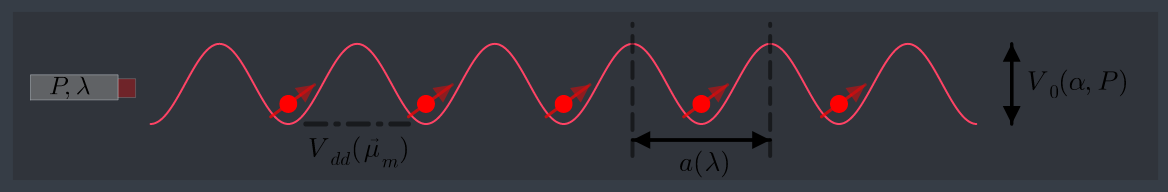
\includegraphics[width=\textwidth]{ch1/mapping.png}
    \end{subfigure}
    \caption{Pictorial representation of ultracold bosons in an optical lattice}
    \label{fig:optical_lattice}
\end{figure}
%%% FIG %%%
\FloatBarrier \!\!\!\!\!\!\!\!\!\!\!

This is, of course, an incredibly simple picture of the setup and there are many more experimentally relevant details that we do not bother with as they do not affect the explorations performed in this thesis. The interested reader may refer to Rudolf et. al. (1999)\cite{grimm1999optical} for a detailed exposition on optical dipole traps for neutral atoms.

\subsection*{Outline of the thesis}

In \autoref{ch1}, we review the basic concepts of a quantum particle trapped in a periodic potential. We introduce the ideas of quasi-momentum, Bloch waves and Wannier functions accompanied with numerical solutions for a particular periodic potential.
\\

In \autoref{ch2}, we proceed to extend our framework to describe the system of interacting bosons in a periodic lattice, thus deriving the Bose-Hubbard model. We also briefly discuss the procedure to map experimental parameters to our theoretical model.
\\

In \autoref{ch3}, we solve the Bose-Hubbard model using various numerical techniques and study the nature of its ground state phases.
\\

In \autoref{ch4}, we analyze a system of bosons with long-range interactions induced by dipole-dipole coupling. This is done by studying the extended Bose-Hubbard model at the mean-field level, thus identifying a variety of new ground state phases that can be realized in the system.
\\

In \autoref{ch5}, we consider spin-1 bosons on a lattice with contact interactions to understand the effect of the spin-degree of freedom on the ground state phases of the Bose-Hubbard model.
\\

In \autoref{ch6}, we analytically study the phenomenon of mediation through bosons by considering a simple impurity model and computing the effective interactions mediated by a conduction band of bosonic atoms on a lattice.
\\

In \autoref{ch7}, we discuss some attempts at extending our analysis beyond the mean-field level. Specifically, we motivate and present the results obtained by utilizing Quantum Monte Carlo techniques to study the finite-temperature physics of the Bose-Hubbard model.
\\

In \autoref{ch8}, we conclude by providing a summary of the results obtained and talk about future prospects for this line of research. 